\section{Vorlesung 11}
\begin{remark}
Aussage $A(x)$ gilt für alle $x \in \mathbb{R}$ bzw. $x \in \{ a , b\}$\\
Aussage $A(x)$ gilt für alle $x \in \mathbb{R}$ ohne $ M$ bzw. $x \in \{ a , b \}$ ohne $\underbrace{M}_{Nullmenge} $\\
kurz: $A(x)$ gilt für $\underbrace{\text{fast alle}}_{\text{fast überall} }$ $x \in \mathbb{R}$ bzw. $x \in \{ a , b\} $  
\end{remark}
\begin{definition}[Nullmenge]
Die Menge $M \subseteq \mathbb{R}$ heißt \textbf{Nullmenge}, wenn gilt :\\
für alle $\epsilon > 0$ existiert Intervalle $ ]_1 , ]_2 , \dots \subseteq \mathbb{R}$ sodass :\\
1) $$ M \subseteq \bigcup_{k=1}^{\infty} J_k = J_1 \cup J_2 \cup \dots $$\\
2) $ \sum_{k=1}^{\infty}|J_k| \leq \epsilon$ wobei $|J_k|$ die Lage des Intervalls $J_k$ bezeichnet.
\end{definition}
\begin{remark}
ab zählbar viele Intervalle endlich viele
ab zählbar unendlich viele
\end{remark}
\begin{example}[1] 
Die Menge $ M = \{ x_1 , x_2 , x_3 \}, |M| = 3$ Die Behauptung : M ist eine Nullmenge .  
\end{example}
\begin{proof}
Sei $\epsilon > 0 $ beliebig und fest 
wähle $J_k$ = $[x_k - \frac{\epsilon}{6}, x_k + \frac{\epsilon}{6}]$
Dann gilt : $|\exists_k|=\frac{\epsilon}{3}$  $x_k \in J_k$ und (1) , (2).
\end{proof}  
\begin{remark}
Endliche Mengen sind Nullmenge.
\end{remark}
\begin{remark}
Abzählbar endliche Mengen sind Nullmengen.
\end{remark}
\begin{proof}
Sei $ M = \{ x_1 , x_2 , x_3 , \dots \}$ und sei $\epsilon > 0 $ beliebig und fest.\\



[ Dann :fehlende Skizze !!! ]
\end{proof}
\textbf{Gesamtlänge berechnen}
\begin{align*}
\sum_{k=1}^{\infty}{\frac{\epsilon}{2^k}} &= \epsilon \sum_{k=1}^{\infty}{\frac{1}{2^k}}\\
&= \epsilon (\dfrac{1}{1-\frac{1}{2}}-1)\\
&= \epsilon(2-1)= \epsilon
\end{align*}
Intervalle $J_k = [x_k - \dfrac{\epsilon}{2^{k+1}}, x_k + \dfrac{\epsilon}{2^{k+1}}](k=1,2,\dots)$ erfüllen (1)und (2).
\begin{remark}
Es gilt überabzählbar Mengen , die Nullmenge sind \textbf{Z.B} die \textbf{[Cantor-Menge]}.

\begin{figure}
	
\centering
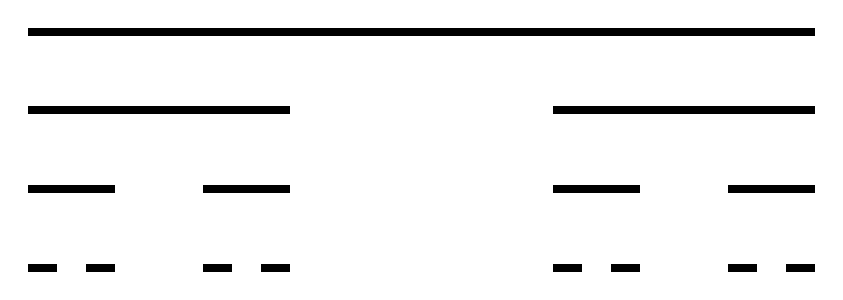
\begin{tikzpicture}[xscale=10,yscale=1]
\def\gen|#1|
{
	\if 0#1
	\path[fill] (0,0) rectangle (1,.1) ;
	\else
	\begin{scope}[xscale=1/3,yshift=-1cm]
	\pgfmathtruncatemacro{\k}{#1-1}
	\gen|\k|
	\begin{scope}[xshift=2cm]
	\gen|\k|
	\end{scope}
	\end{scope}
	\fi
}
\foreach \k in {0,...,3}
{
	\gen|\k|
}


\end{tikzpicture}
	\caption{cantor-Menge}
	die nicht gelöchte punkte bilden die Cantor-Menge
\end{figure}


\end{remark}
\begin{definition}[Cantor-Menge]
Unter der Cantor-Menge versteht man in der Mathematik eine bestimmte Teilmenge der Menge der reellen Zahlen.\\
\textbf{Schnitte von Intervallen}\\
Die Cantormenge lässt sich mittels folgender Iteration konstruieren:
Man beginnt mit dem abgeschlossenen Intervall $[0,1]$ der reellen Zahlen von 0 bis 1. 
\end{definition}
\[ \int_{a}^{b} f(x) dx = \int_{a}^{c} f(x) dx + \int_{c}^{b} f(x) dx \text{ für alle } x \in \mathbb{R} \]
\begin{definition}
$$ \int_{b}^{c} f(x) dx = - \int_{c}^{b} f(x) dx $$ 
\end{definition}
\subsection{Mittelwertsatz der Integralrechnung}
Sei $f : [a,b]$ stetige Funktion  dann existiert ein $ z \in [a,b]$ mit $\int_{a}^{b} f(x) dx = f(z) \times (a-b)$\\ \\
\begin{tikzpicture}
\begin{axis}[
axis y line = left,
axis x line = middle,
xtick       = {0,2,3.8},
xticklabels = {$b$,$x$,$a$},
ytick       = {3},
yticklabels = {$f(x)$},
samples     = 160,
domain      = 0:3.8,
xmin = -1, xmax = 5,
ymin = -5, ymax = 10,
]
\addplot[name path=poly, black, thick, mark=none, ] {-x^3+5*(x^2)-3*x+0.5};
\addplot[name path=line, gray, no markers, line width=1pt] {3};
\draw [thick, brown, decorate,decoration={brace,amplitude=10pt,mirror},xshift=0.4pt,yshift=-10pt](0,-1) -- (3.8,-1) node[black,midway,yshift=-0.6cm] {\footnotesize $b-a$};
\addplot fill between[ 
of = poly and line, 
split, % calculate segments
every even segment/.style = {orange!70},
every odd segment/.style  = {gray!60}
];
\end{axis}
\end{tikzpicture}

\subsection{Hauptsatz der Differenzial und Integralrechnung }
Sei $ f : [a , b] \rightarrow \mathbb{R} $ ein stetige Funktion , und sei $ \widetilde{F} : [a , b] \rightarrow \mathbb{R	}$ . $ x \longmapsto \int_{a}^{x} f(t) dt $
Dann ist $\widetilde{F}$ auf $(a,b)$ differenzierbar  und es gilt $\widetilde{F}'$ für alle $x \in (a , b)$
\begin{proof}
Sei $x_0 \in (a,b)$ beliebig und fest 
\begin{align*}
\widetilde{F}'(x_0) &= \lim_{x \to x_0 }{\frac{\widetilde{F}(x)-\widetilde{F}(x_0)}{x - x_0}}\\
&= \lim_{x \to x_0 }{\dfrac{\int_{a}^{x} f(t) dt - \int_{a}^{x_0} f(t) dt}{x - x_0}}\\
&= \lim_{x \to x_0 }{\dfrac{\int_{a}^{x_0} f(t) dt + \int_{x_0}^{a} f(t) dt - \int_{a}^{x_0} f(t) dt}{x - x_0}}\\
&= \lim_{x \to x_0 }{\dfrac{\int_{x_0}^{x} f(t) dt}{x -x_0}}
\end{align*}
laut \textbf{Mittelwertsatz} existiert $z \in (x_0,x)$ mit
\begin{align*} 
 \widetilde{F}'(x_0) &= \lim_{ z \to x_0}{\frac{f(z)( x - x_0 )}{ x - x_0}}\\
&= \lim_{z \to x_0}{f(z)} \underbrace{=}_{\text{f ist stetig}} f(x_0) 
\end{align*}
\end{proof}
\begin{remark}
$\widetilde{F}$ ist eine spezielle Stammfunktion.
\end{remark}
\begin{definition}[Stammfunktion]
eine Funktion heißt \textbf{Stammfunktion} zu $f(x)$ im Intervall $(a , b)$ , wenn gilt :
\[ F'(x) = f(x) \text{ für alle } x \in (a , b) \]
\end{definition}
\begin{remark}
\begin{align*}
F'_1(x) = F'_2(x) = f(x) &\Rightarrow 
F'_2(x)-F'_1(x) = 0\\
&\Rightarrow (F_2(x) - F_1(x))'=0 \text{ für alle  } x \in (a,b) \quad \big\} f_2(x) - f_1(x) = c const\\
&\Rightarrow F_2(x) = F_1(x) + c , \quad c \in \mathbb{R}
\end{align*}
\end{remark}
\begin{definition}
Die Mengen aller Stammfunktion $F(x)$ zu $f(x)$ heißt \textbf{unbestimmtes Integral}.
\end{definition}
\begin{remark}[unbestimmtes Integral]
Das unbestimmte Integral ist \textbf{kein} Integral.\\
\subsection{Schreibweise}
\[ \int f(x)dx = \{ F(x) | F'(x) = f(x) \} \]
bzw
\[ \int {f(x)dx} = F(x) + c , \quad c \in \mathbb{R} \text{ falls  } F'(x) = f(x) \] 
\end{remark}
\subsection{2. Hauptsatze der Differenzial- und Integralrechnung}
Sei $f:[a ,b] \rightarrow \mathbb{R}$ und $f$ stetig\\
Sei $F(x)$ eine Stammfunktion zu $f$ , Dann gilt
\[ \int_{a}^{b} f(x) dx = F(b)-F(a) \]

	\centering
	\begin{tikzpicture}[scale=1.3],\begin{axis}[
	axis y line = left,
	axis x line = bottom,
	xtick       = {-0.5,1},
	xticklabels = {$b$,$a$},
	ytick       = \empty,
	samples     = 160,
	domain      = -0.5:2,
	xmin = -4, xmax = 4,
	ymin = 0, ymax = 3,
	]

	\addplot[color=red,domain=-4:4,samples=100] {sqrt(2*pi)*exp(-x^2/2)};

	\addplot[color=red,fill=red, pattern=north east lines,  domain=-0.5:1,samples=100] {sqrt(2*pi)*exp(-x^2/2)} \closedcycle;

	\end{axis}
	\end{tikzpicture}

\begin{proof}
\begin{align*}
\underbrace{\int_{a}^{b} f(x)dx}_{:= f(t)dt} = \i\underbrace{\int_{a}^{b} f(t)dt}_{\widetilde{F}(b)} - \underbrace{\int_{a}^{a} f(t)dt}_{\widetilde{F}(a)}\\
\textbf{ Note! }\widetilde{F}(x) = F(x) + c \quad: c \in \mathbb{R}\\
 = (F(b)+c) - (F(a)+c) = F(b)- F(a)
\end{align*}
\end{proof}
\begin{remark}
\begin{gather*}
f \underbrace{\longrightarrow}_{ableiten} f'\\
f' \underbrace{\longrightarrow}_{integrieren} f \\
\int {f'(x)dx} = F(x) + c  \quad c \in \mathbb{R}
\end{gather*}
\begin{example}
\begin{gather*}
\int{x^k dx} = \frac{x^{k+1} }{ k+1 } + c , \quad c \in \mathbb{R}\\
\int{\frac{1}{1+x^2}dx} = arctan(x) + x , \quad c \in \mathbb{R}
\end{gather*}
\end{example}
\end{remark}
\subsection{Integrationsregeln entstehen aus Ableitungsregeln}
\begin{enumerate}
\item \[(F(x) + G(x))' = F'(x) + G'(x) \Rightarrow \int f(x)dx + \int g(x)dx. \] 
\item \[\int K \times f(x)dx = K \int f(x)dx \]
\item \[\bigg( \frac{1}{a} \times F(ax+b)\bigg)'=\frac{1}{a} \times F'(ax+b)\times a = F'(ax+b)\]
\item \[ \int F' (ax+b) dx = \frac{1}{a} \times F(ax+b)+ c , \quad c \in \mathbb{R} \]
\end{enumerate}